\documentclass{ximera}

%\documentclass{ximera}

\usepackage{float}
\usepackage{subcaption}

\pgfplotsset{compat=1.16}

\newtheorem{ass}{Assumption}

\def\check{\tikz\fill[scale=0.4](0,.35) -- (.25,0) -- (1,.7) -- (.25,.15) -- cycle;}





\outcome{Know how to measure the return on an investment.}

\author{Brad Waller}

%Section 1.4

\title{Measuring Returns}

\begin{document}

\begin{abstract}
Returns are the measuring stick of the investment world. It is importand to be able to compare two assets, and the value of the assets is not always preferred.
\end{abstract}

\maketitle

People invest in financially risky assets so that they can yield the reward of higher returns. The objective is to exceed the return that would be received by investing money in a risk-free government bond. To ensure that you exceed the risk-free rate, it is necessary to measure returns. There are three ways that we will measure returns, and they are all beneficial in some way. They are

\begin{enumerate}
\item payoff,
\item profit,
\item and rate of return. 
\end{enumerate}

The first is perhaps the least useful for measuring a return; however, it is extremely useful going forward. We will almost exclusively use payoffs to determine the price of a class of investments called {\bf derivatives}. These will be seen in the upcoming sections with a formal definition.

Profit and rate of return are very useful in measuring return. It may inspire curiousity as to why there are two. Profit indexes your payoff against the opportunity cost of your investment. Rate of return answers the question, ``what rate of return would my initial investment have needed to arrive at a specified payoff?" More formally, the definitions for each are provided in below.

\begin{definition}\label{def9}
The {\bf payoff}\index{payoff} of a financial position at time $T$ is the amount of money you could walk away with if you liquidated your position. The {\bf profit}\index{profit} of a financial position at time $T$ is the difference of your payoff and your initial investment grown at the risk-free rate. The {\bf rate of return}\index{rate of return} of a financial position at time $T$ is the continuously compounded rate of return that would grow your initial investment to your payoff. 
\end{definition}

\begin{remark}
In the event that the financial position is worth nothing, one might say that the rate of return is $-\infty$. Also, we will usually compute rate of return when dealing with a positive investment. 
\end{remark}

Let's see our definitions in action!

\begin{example}
You purchased 100 shares of stock in a company two years ago for $25$/share. The dividend rate is 2\%, and the risk-free rate is 6\%. Today, the price/share of your investment is $28$/share. Determine the payoff, profit, and rate of return on your investment.

\end{example}

\begin{solution}
We'll proceed in order. The payoff is the vaue of the investment after 2 years,
	\begin{equation*}
		100e^{0.02\cdot 2}\cdot 28=2914.27.
	\end{equation*}
The profit is the difference of the payoff and the opportunity cost of the initial investment,
	\begin{equation*}
		2914.27-25\cdot 100e^{0.06\cdot 2}=95.53
	\end{equation*}
The rate of return is the rate required to grow the initial investment to the payoff,
	\begin{align*}
		25\cdot 100e^{\alpha\cdot 2}&=2914.27\\
		\alpha&=0.077
	\end{align*}
\end{solution}


\begin{remark}
Observe that the quantity of shares in the previous example influences the payoff and the profit; however, it has no effect on the rate of return. If you aren't convinced, double the quantity of shares involved and recompute everything in the example.
\end{remark}

Payoffs will be {\bf the most important aspect of a derivative} when determining the price of the derivative. A great tool in building our intuition will be payoff and profit diagrams. Suppose that in our previous example, we only purchased one share initially. The 25 we paid initially would be at time 0, and the payoff is at time 2. When we are at time 0, our payoff at time 2 is unknown; the payoff is a variable dependent on the value $S(2)$. In fact, we can write it as a function: $S(2)e^{0.02\cdot 2}$. The profit is similar; it is the payoff shifted down. $S(2)e^{0.02\cdot 2}-25e^{0.06\cdot 2}$. The difference comes from the opportunity cost consideration. The graphs for payoff and profit are given below.

%\begin{figure}[H]
%	\begin{subfigure}{.4\linewidth}
%	\centering
\begin{center}
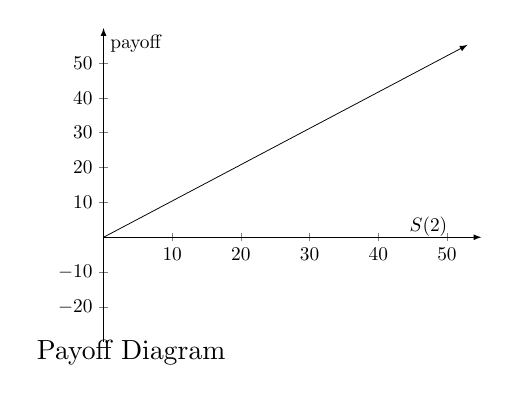
\begin{tikzpicture}[scale=0.7]
	\begin{axis}[
		xmin=0,
		xmax=55,
		xtick={10,20,...,50},
		ymin=-30,
		ymax=60,
		ytick={-20,-10,...,50},
		%grid=both,
		axis lines=middle,
		axis line style={->, >=latex},
		x label style={at={(axis description cs:0.86,0.42)},anchor=north},
		xlabel={$S(2)$},
		ylabel={payoff}]
		%style={font=\tiny}]
		\addplot[black, smooth, domain=0:53, ->, >=latex]{x*1.04081};
	\end{axis}
	\node at (0.5, -0.2){Payoff Diagram};
\end{tikzpicture}
\hspace{10pt}
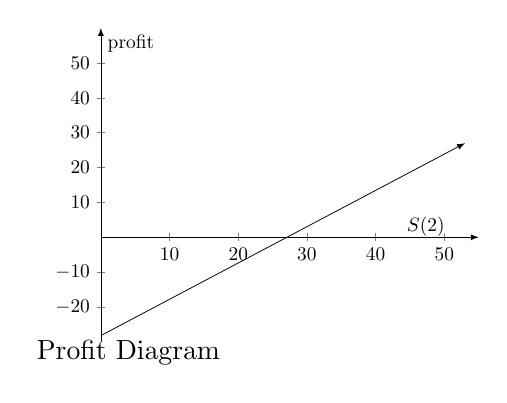
\begin{tikzpicture}[scale=0.7]
	\begin{axis}[
		xmin=0,
		xmax=55,
		xtick={10,20,...,50},
		ymin=-30,
		ymax=60,
		ytick={-20,-10,...,50},
		%grid=both,
		axis lines=middle,
		axis line style={->, >=latex},
		x label style={at={(axis description cs:0.86,0.42)},anchor=north},
		xlabel={$S(2)$},
		ylabel={profit}]
		%style={font=\tiny}]
		\addplot[black, smooth, domain=0:53, ->, >=latex]{x*1.04081-28.19};
	\end{axis}
	\node at (0.5, -0.2){Profit Diagram};
\end{tikzpicture}
%	\caption{Profit Diagram}
%	\end{subfigure}
%	\caption{Payoff and Profit}
%\end{figure}

\end{center}

The picture for profit is the motivation for the term {\bf break-even value}\index{break-even value}. The break-even value of an investment is the value(s) of the underlying asset that would yield a profit of 0. For our diagram, the break-even value for $S(2)$ is approximately 27.08. 

\begin{question}
You invest in ZYX. The value today is \$120, the dividend rate is $r=0.07$, and the risk-free rate is $\delta=0.02$. What value would ZYX need to take in one year so that you broke even on your investment?
	\begin{prompt}
		$\text{The share's value is}=\answer{126.15}$
	\end{prompt}	
\end{question}

\begin{solution}
The solution is short, but it takes some thought to get to the correct result. The quantity invested does not matter, so we may as well assume that one share was purchased initially. After one year, you will have dividend growth in the quantity of shares, so your investment will look like
	\begin{equation*}
		S(1)e^{0.02}
	\end{equation*}
You also know that you could have invested your \$120 at the risk-free rate. That would give you
	\begin{equation*}
		120e^{0.07}
	\end{equation*}
The result follows when you equate the two.
	\begin{align*}
		S(1)e^{0.02}&=120e^{0.07}\\
		S(1)&=120e^{0.07-0.02}=126.15
	\end{align*}
\end{solution}

The value in the previous question has a special name: it is the forward price of ZYX. Let's make the following definition.

\begin{definition}\label{def10}
The time $T$ {\bf forward price} of an asset $S$ at time $t$ is denoted 
	\begin{equation*}
		F_{t,T}(S).
	\end{equation*}
The value is given by 
	\begin{equation*}
		S(t)e^{(r-\delta)(T-t)}.
	\end{equation*}
\end{definition}

\begin{remark}
In our normal context, we will be talking about an investment today and at some particular point in the future. When these values are understood, we will just say the forward price. That is how we used it after the question, and it is the least awkward when we speak about such things in the future. The value would look different if we permitted discrete dividends.
\end{remark}

\end{document}




